%-------------------------------------------------------------------------------
\documentclass[a4paper, 12pt] {article}
%-------------------------------------------------------------------------------
\usepackage[brazil]{babel}
\usepackage[utf8]{inputenc}
\usepackage{graphicx}
\usepackage[none]{hyphenat}
\usepackage{indentfirst}
\usepackage{setspace}
\usepackage{comment}
\usepackage{amsmath}
\usepackage[numbers]{natbib}
\usepackage{hyperref}
%-------------------------------------------------------------------------------
\newcommand{\p}{$\bullet$}
%-------------------------------------------------------------------------------
\addtolength{\hoffset}{-1.5cm}
\addtolength{\voffset}{-2.0cm}
\addtolength{\textwidth}{3.0cm}
\addtolength{\textheight}{4.1cm}
%-------------------------------------------------------------------------------
\sloppy
%------------------------------------------------------------------------------
\begin{document}

\thispagestyle{empty}
\begin{center}

\vskip 2.2cm

\Large{Título: Algoritmos Multi-BSP para o problema da submatriz de tamanho
máximo 3D}

\vskip 1.5cm

\Large{Projeto de Pesquisa}

\vskip 1.5cm

\Large{Projeto de Pesquisa apresentado como exigência da primeira fase do
processo seletivo para ingresso no programa de Pós-Graduação em Ciência
da Computação, nível Doutorado, promovido entre a Universidade
Federal de Mato Grosso Sul e a Universidade Federal de Goiás.}

\vskip 2.5cm

\Large{Rodrigo Gonçalves de Branco}

\vskip 2.0cm

%{\Large Orientador:}

\vskip 2.5cm

\large{Programa de Pós-Graduação em Ciência da Computação, nível de Doutorado,
da Faculdade de Computação da UFMS em associação com o Instituto de Informática da UFG}

\vskip 1.3cm

Campo Grande--MS, outubro de 2014

\end{center}

\clearpage
%-----------------------------------------------------------------
\onehalfspacing
%-------------------------------------------------------------------------------
\pagenumbering{arabic}

\section{Introdução}

O problema da subsoma de tamanho máximo pode ser definido como: dado um conjunto
de $n$ números reais, a subsoma de tamanho máximo é a maior soma contígua de
elementos, dentre todas as somas contíguas possíveis no conjunto
dado \cite{bentley2000programming}. A Figura \ref{fig:maxsubsum} apresenta um
exemplo do problema citado e as possíveis soluções.
Este problema pode ser encontrado em diversas áreas, como Biologia Computacional, principalmente na localização de segmentos biológicos significantes e identificação de domínios
transmembranos em uma sequência de proteínas \cite{bae2007}. Jay Kadane
apresentou um algoritmo de complexidade $O(n)$ para resolver o problema descrito, utilizando 
programação dinâmica \cite{bentley2000programming}.

\begin{figure}[ht]
\centering
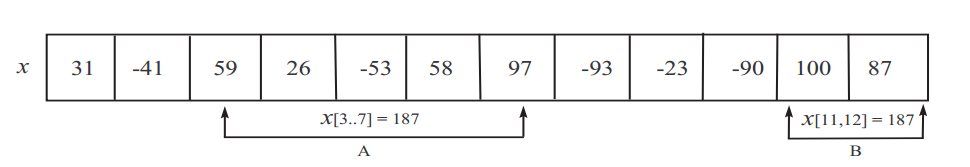
\includegraphics[width=.8\textwidth]{maxsubsum.png}
\caption{Vetor com 12 elementos, com duas subsomas de tamanho máximo.}
\label{fig:maxsubsum}
\end{figure}

Este problema pode ser estendido para duas dimensões. A motivação para este problema pode ser
encontrada em áreas como visão computacional, identificando em imagens (sejam
elas de áreas médicas, de astronomia, termais, entre outras) as regiões de
interesse. Dado uma matriz de $nxn$
números reais, a submatriz de soma máxima é a maior submatriz retangular cuja
soma de seus elementos apresenta a soma máxima, dentre todas as submatrizes
possíveis no conjunto de entrada apresentado. A Figura \ref{fig:maxsubarray}
apresenta um exemplo para este problema e a Figura \ref{fig:brightest} apresenta
um exemplo desta aplicação.

\begin{figure}[ht]
\centering
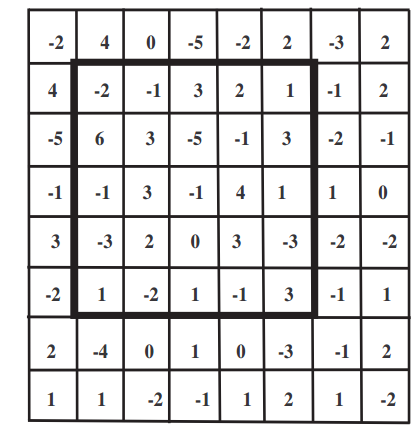
\includegraphics[width=.35\textwidth]{maxsubarray.png}
\caption{A região destacada é submatriz de soma máxima para a matriz
apresentada.}
\label{fig:maxsubarray}
\end{figure}

\begin{figure}[ht]
\centering
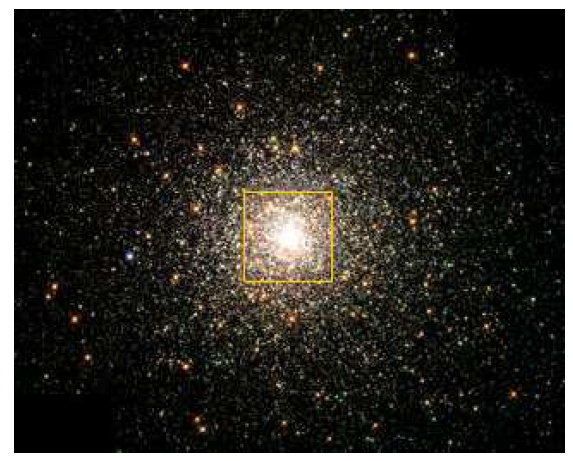
\includegraphics[width=.4\textwidth]{brightest.png}
\caption{Área mais brilhante em uma imagem de astronomia \cite{bae2007}.}
\label{fig:brightest}
\end{figure}

O algoritmo linear proposto por Kadane pode ser extendido para resolver a versão
2D. A matriz de entrada é substituida pela soma de prefixo de suas linhas, e com
essa nova matriz, a submatriz de soma máxima é então calculada da seguinte
forma: para cada par de colunas possíveis (denominadas $Cgh$, tal que $1 <= g
<= h <= n$), o algoritmo linear de Kanade é usado para, naquela configuração de
colunas, encontrar a maior soma daquela configuração, delimitando portanto as linhas da matriz considerada. Assim, para
uma matriz com $nxn$ elementos, é necessário calcular $\frac{n(n-1)}{2} Cgh's$,
e cada um deles utiliza $O(n)$ passos para encontrar a submatriz de soma máxima
para aquela configuração. Portanto, o algoritmo resultante possui complexidade
$O(n^3)$.

\subsection{Algoritmos Paralelos}

Em função do volume de dados das aplicações descritas anteriormente, as
versões apresentadas, executando em computadores tradicionais sequenciais, podem
não apresentar os resultados dentro de um período de tempo satisfatório. Por
esse motivo, algoritmos paralelos em diversos modelos foram
apresentados para minimizar este problema.

\subsubsection{PRAM}

O modelo PRAM (\textit{Parallel Random Access Machine}) é uma máquina paralela
abstrata utilizada para modelar algoritmos paralelos teóricos que teriam um
comportamento previsível em termos assintóticos em computadores paralelos reais.
A vantagem do modelo PRAM é que ele ignora questões como comunicação entre os
processadores, permitindo que seu utilizador foque no potencial paralelismo do
algoritmo proposto. Os processadores não estão diretamente interligados entre
si, mas possuem acesso a uma memória global, onde podem trocar informações. A
Figura \ref{fig:pram} apresenta uma representação visual do modelo PRAM. 

\begin{figure}[ht]
\centering
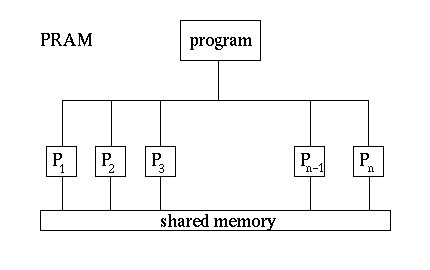
\includegraphics[width=.4\textwidth]{pram.png}
\caption{Modelo PRAM (Fonte:
\url{http://www.cs.uku.fi/~penttone/parallel/pram.html}) }
\label{fig:pram}
\end{figure}

Para deixar o modelo PRAM um pouco mais realístico, é possível especificar a
forma de acesso à memória, a fim de evitar conflitos de região crítica e condições de
corrida. As estratégias são:

\begin{itemize}
  \item EREW (\textit{Exclusive read exclusive write}) - cada posição de memória
  deve ser lida ou escrita por apenas um processador de cada vez;
  \item CREW (\textit{Concurrent read exclusive write}) -  vários processadores
  podem ler uma posição de memória ao mesmo tempo, mas apenas um processador
  pode escrever na mesma de cada vez;
  \item ERCW (\textit{Exclusive read concurrent write}) - vários processadores
  podem escrever em uma posição de memória ao mesmo tempo, mas apenas um
  processador pode lê-la de cada vez;
  \item CRCW (\textit{Concurrent read concurrent write}) - vários processadores
  podem ler e/ou escrever ao mesmo tempo.
\end{itemize}

Quando nada é dito sobre um algoritmo PRAM, neste trabalho é assumido que ele
utiliza a estratégia EREW, por ser mais próxima das arquiteturas existentes.

É possível encontrar algoritmos, tanto para o problema 1D quanto para o 2D,
descritos no modelo PRAM. Em \cite{journals/ppl/PerumallaD95}, para o problema
1D, um dos algoritmos  possui complexidade $O(log n)$, utilizando $O(\frac{n}{log
n})$ processadores. Para o problema 2D, o algoritmo apresentado também possui
complexidade $O(log n)$, utilizando $O(\frac{n^3}{log
n})$ processadores.

\subsubsection{BSP}

Leslie Valiant propôs o modelo BSP (\textit{Bulk Synchronous
Parallel}), com o objetivo de aproximar o
desenvolvimento de algoritmos paralelos para
arquiteturas reais \cite{Valiant:1990:BMP:79173.79181}. Este modelo não garante
comunicação e sincronização, e estes fatores devem ser considerados no projeto
de um algoritmo BSP. A Figura \ref{fig:bsp} apresenta um superpasso de um
algoritmo BSP.

\begin{figure}[ht]
\centering
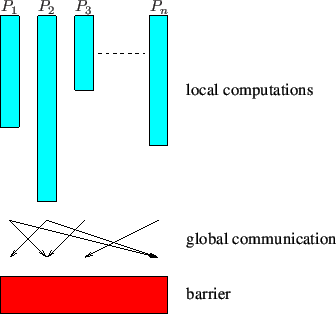
\includegraphics[width=.4\textwidth]{bsp.png}
\caption{Modelo BSP (Fonte:
\url{http://ww2.cs.mu.oz.au/~aaron/subjects/comp90025_2011_sm2/lectures/node195.html}) }
\label{fig:bsp}
\end{figure}

O modelo BSP pode ser combinado com o modelo CGM (\textit{Coarse Grained
Multicomputer}, exemplificado pela Figura \ref{fig:cgm}), este último
apresentado por Dehne \textit{et al} \cite{Dehne:1993:SPG:160985.161154}, em situações em que a entrada do problema é
muito maior que o número de processadores disponíveis. Um algoritmo CGM típico
consiste de uma sequência de rodadas, alternando entre etapas de computação e
comunicação separados por barreiras de comunicação.

\begin{figure}[ht]
\centering
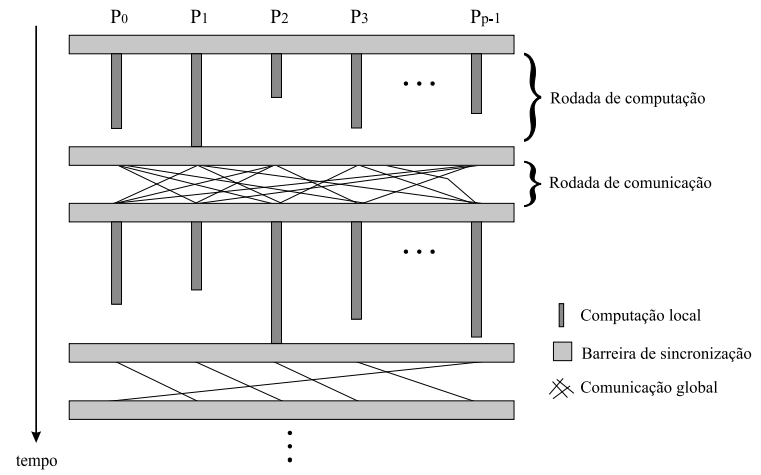
\includegraphics[width=.6\textwidth]{cgm.png}
\caption{Modelo CGM \cite{loureiro2010}. }
\label{fig:cgm}
\end{figure}

Alves \textit{et al} apresentam algoritmos BSP/CGM tanto para o problema 1D
quanto para o problema 2D \cite{alves2004}. O problema 1D é resolvido
com $p$ processadores, com tempo de computação local igual a  $O(\frac{n}{p})$ e $O(1)$
rodadas de comunicação. A solução do problema 2D difere do problema 1D no tempo
de computação local, pois este é igual a $O(\frac{n^3}{p})$.

\subsubsection{Multi-BSP}

O surgimento de arquiteturas \textit{multicore} e \textit{manycore} despertou o
interesse na implementação de algoritmos em plataformas
híbridas. Com essa perspectiva, Valiant apresentou o modelo Multi-BSP
\cite{Valiant:2008:BMM:1431008.1431011}, modelo este que explicita parâmetros
como número de processadores, tamanho de memória e cache, custos de comunicação
e sincronização.

A resolução dos problemas 1D e 2D para este modelo normalmente são apresentadas
em nível de implementação com demonstrações de \textit{speedup} em relação às
implementações já conhecidas na literatura, apresentados principalmente para os
modelos PRAM e BSP/CGM \cite{6473291,doi:10.1117/12.928318,takaoka2014efficient}.

\subsection{Bibliotecas e implementações Paralelas}

A efetividade dos algoritmos propostos é comprovada através de implementação dos
mesmos em alguma arquitetura disponível, apresentando o \textit{speedup} em
relação ao algoritmo sequencial tradicional, quando esta implementação é
possível. A seguir serão apresentadas as principais bibliotecas para
implementação de soluções paralelas.

\subsubsection{OpenMP}

A biblioteca OpenMP\footnote{\url{http://openmp.org/wp/}} permite o paralelismo
em através de memória compartilhada com utilização de \textit{threads} (que atuam
como os processadores dos algoritmos teóricos) para arquiteturas
\textit{multicore}. A comunicação entre os processadores é feita via memória
compartilhada, ficando sob responsabilidade do programador tratar de questões como regiões críticas e
condições de corrida. Portanto, um processo é iniciado e dentro dele
\textit{threads} são criadas para resolver um problema em comum. A Figura
\ref{fig:openmp} apresenta a divisão e união das \textit{threads} para a
resolução do problema utilizando a biblioteca OpenMP.

\begin{figure}[ht]
\centering
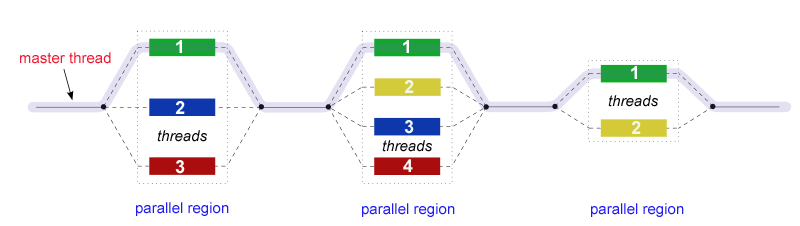
\includegraphics[width=.6\textwidth]{fork_join2.png}
\caption{Explicitação das regiões paralelas utilizando \textit{threads} com a
biblioteca OpenMP (Fonte: \url{https://computing.llnl.gov/tutorials/openMP/})}
\label{fig:openmp}
\end{figure}

\subsubsection{MPI}

O modelo BSP/CGM pode ser facilmente mapeado e implementado utilizando
bibliotecas que implementam o padrão MPI (\textit{Message Passing
Interface})\footnote{\url{https://computing.llnl.gov/tutorials/mpi/}}.
Utilizando este padrão, os processadores são tipicamente interligados através de uma rede de
comunicação, cada um com sua memória local, e a comunicação é feita através da
troca explícita de dados entre eles. O conjunto de processadores formam então um
\textit{cluster}, onde as aplicações podem ser executadas. É interessante
destacar que as máquinas que compõem o \textit{cluster} podem ser ser de
diferentes arquiteturas, com diferentes sistemas operacionais, tendo em comum o
programa a ser executação e o padrão e protocolo de comunicação entre elas. A
Figura \ref{fig:mpi} apresenta a estrutura de comunicação de sistemas que usam o
padrão MPI.

\begin{figure}[ht]
\centering
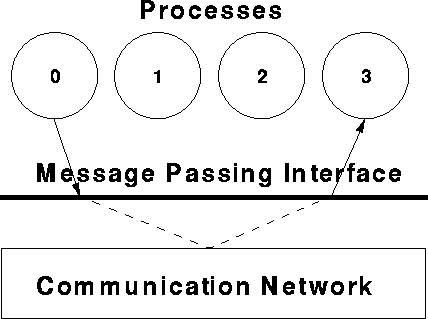
\includegraphics[width=.35\textwidth]{mpi.png}
\caption{Modelo de comunicação MPI (Fonte:
\url{http://nf.nci.org.au/training/MPIProg/slides/allslides.html})}
\label{fig:mpi}
\end{figure}

\subsubsection{GPGPU}

Por fim, a popularização de dispositivos GPGPU (\textit{General Purpose Graphics
Processing Unit}), devido a velocidade de processamento e número de
processadores, despertou a atenção dos pesquisadores para a implementação de
algoritmos paralelos para esta arquitetura. Os processadores das placas gráficas, conhecidos como dispositivo GPU, possuem
alguns SM (\textit{Stream Multiprocessor}), que executam um conjunto de blocos, e estes
por sua vez executam um conjunto de \textit{threads}. A comunicação entre as
\textit{threads} é feita através da memória global do dispositivo, e a
sincronização entre blocos é feita através do lançamento de \textit{kernels},
unidade básica de configuração de uma rodada de execução. Implementações
conhecidas de programação GPGPU são CUDA (\textit{Compute Unified Device
Architecture})\footnote{\url{http://www.nvidia.com.br/object/cuda_home_new_br.html}}
e OpenCl (\textit{Open Compute
Language})\footnote{\url{https://www.khronos.org/opencl/}}. A Figura
\ref{fig:cuda-arranje} apresenta a organização de um multiprocessador da
arquitetura CUDA, enquanto a Figura \ref{fig:cuda-execution} apresenta o modelo
simplificado de \textit{threads} CUDA.

\begin{figure}[ht]
\centering
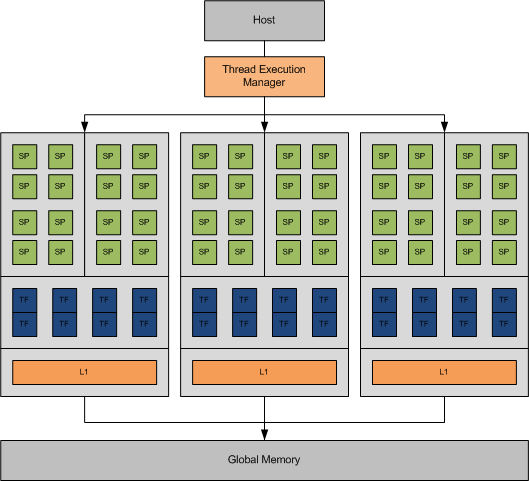
\includegraphics[width=.4\textwidth]{cuda-arranje.png}
\caption{Organização de um Multiprocessador CUDA (Fonte:
\url{http://wiki.expertiza.ncsu.edu/index.php/CSC/ECE_506_Spring_2011/ch2a_mc}) }
\label{fig:cuda-arranje}
\end{figure}

\begin{figure}[ht]
\centering
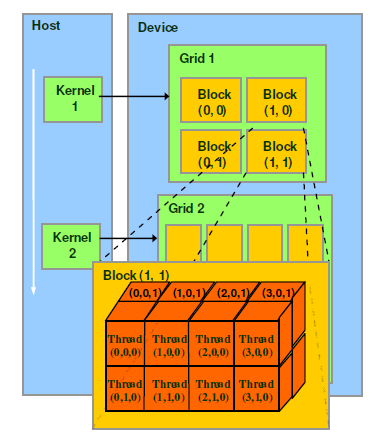
\includegraphics[width=.4\textwidth]{Cuda_execution.png}
\caption{Modelo de Threads CUDA (Fonte:
\url{http://wiki.expertiza.ncsu.edu/index.php/CSC/ECE_506_Spring_2011/ch2a_mc}) }
\label{fig:cuda-execution}
\end{figure}


\subsubsection{Mapeamento de modelos para implementações}

Nem sempre é possível implementar diretamente um algoritmo descritos nos modelos
PRAM, BSP, BSP/CGM ou mesmo Multi-BSP diretamente para uma arquitetura alvo.
Detalhes e limitações como número de processadores, tamanho de memória e forma
de comunicação e sincronização pode forçar a mudanças no algoritmo para
adequá-lo a realidade da arquitetura, podendo resultar em um algoritmo
completamente novo para um problema já conhecido.

\subsection{O problema 3D}

Perumalla e Deo indicam que os problemas 1D e 2D
podem ser generalizados para $d$ dimensões, da seguinte forma: dado um cubo $d-$dimensional com lado de tamanho $n$ de números reais,
encontre o sub$-d-$cubo que possui a maior soma de todos os sub$-d-$cubos
possíveis \cite{journals/ppl/PerumallaD95}. Usando a mesma estratégia da versão
2D descrita anteriormente, é possível descrever um algoritmo para resolver o problema $n-$dimensional. O
algoritmo PRAM sugerido para um $d-$cubo com lado de tamanho $n$ pode ser
computado em $O(log n)$, usando $n\binom{n}{2}^{d-1}$ processadores.

Partindo da motivação de localização de áreas de interesse em uma imagem médica,
podemos estender essa análise para modelos médicos 3D, gerados por exemplo, a
partir de uma ressonância magnética. Dessa forma, a resolução do problema 3D se
mostra atrativa. Contudo, o algoritmo sequencial 3D conhecido tem complexidade
$O(n^5)$, enquanto a versão PRAM verificada precisa de $O(n^5)$ processadores.

Não foram encontrados na literatura algoritmos paralelos para a versão
3D, tampouco implementações paralelas para resolução deste problema.


\section{Objetivos}

O principal objetivo deste trabalho é estudar e obter algoritmos Multi-BSP
para resolver a versão 3D do problema da submatriz de soma máxima. A versão sequêncial deste
problema possui complexidade $O(n^5)$, tornando o algoritmo proibitivamente
custoso, motivando a obtenção de versões paralelas para resolução do problema
dentro de um período de tempo aceitável.

O algoritmo PRAM conhecido não pode ser implementando nas arquiteturas
disponíveis, pois o número de processadores utilizado também é proibitivo. Além
disso, características não incorporadas ao modelo PRAM durante o
desenvolvimento dos algoritmos, tais como custo adicional para referência à memória global e latência, 
têm grande impacto no desempenho das implementações \cite{castro2003}.

As placas gráficas que permitem a programação GPGPU já são otimizadas para
maninular dados em duas e três dimensões, sugerindo que um algoritmo Multi-BSP
direcionados a essa arquitetura pode fornecer bons resultados. Ainda assim, é
importante que outras arquiteturas sejam estudadas, seja para comparar as
estruturas do algoritmo como para comparar os \textit{speedups} obtidos.

\section{Metodologia}

O desenvolvimento do presente projeto estrutura-se nas seguintes atividades:

\begin{enumerate}
  \item complementar a revisão bibliográfica iniciada, detalhando os
  algoritmos, implementações e detalhes que mereçam destaque para o projeto;
  \item estudar as bibliotecas OpenMp, MPI e CUDA/OpenCl, para implementação
  dos algoritmos presentes na literatura;
  \item implementar a solução trivial (ingênua) do problema 3D nas arquiteturas
  descritas;
  \item propôr novos algoritmos Multi-BSP para o problema 3D, apresentando
  estratégias de solução paralela que faça a divisão de:
  	\begin{itemize}
  	  \item dados;
  	  \item computação a ser realizada;
  	  \item ambas;
  	\end{itemize}
  \item implementar os algoritmos propostos nas arquiteturas alvo com as
  bibliotecas mencionadas, ressaltando as diferenças e pecurialidades
  particulares de cada uma delas;
  \item realizar experimentos para avaliar a eficiência das soluções propostas,
  tanto em termos de sua complexidade teórica como performance de implementação
  e execução, comparando com soluções pré-existentes, se existirem.
\end{enumerate}

\section{Etapas e Cronograma}

O cronograma previsto contempla a realização do curso de doutorado e do projeto
aqui descrito e é apresentado na Tabela \ref{tab:cronograma}. O cronograma está
organizado em termos das etapas que consistem em pontos importantes do curso e da execução do projeto.

\begin{table}[htbp]
\begin{center}
\resizebox{\columnwidth}{!}{%
\begin{tabular}{|c|c|c|c|c|c|c|c|c|}
\hline
\multicolumn{ 1}{|c|}{\textbf{Cronograma previsto}} & \multicolumn{ 2}{c|}{\textbf{1º Ano}} & \multicolumn{ 2}{c|}{\textbf{2º ano}} & \multicolumn{ 2}{c|}{\textbf{3º ano}} & \multicolumn{ 2}{c|}{\textbf{4º ano}} \\ \cline{ 2- 9}
\multicolumn{ 1}{|l|}{} & 1º Sem & 2º Sem & 3º Sem & 4º Sem & 5º Sem & 6º Sem & 7º Sem & 8º Sem \\ \hline
Obtenção de Créditos em disciplinas & \p & \p &  &  &  &  &  &  \\ \hline
Revisão da Literatura &  & \p & \p &  &  &  &  &  \\ \hline
Planejamento e modelagem dos algoritmos &  &  & \p & \p &  &  &  &  \\ \hline
Implementação dos algoritmos &  &  &  & \p & \p & \p &  &  \\ \hline
Testes dos algoritmos &  &  &  &  & \p & \p &  &  \\ \hline
Verificação de resultados &  &  &  &  &  & \p & \p &  \\ \hline
Comparação com outras soluções já desenvolvidas &  &  &  &  &  & \p & \p &  \\ \hline
Ajustes e otimização dos algoritmos desenvolvidos &  &  &  &  &  &  & \p &  \\ \hline
Análise e interpretação dos resultados &  &  &  &  &  &  & \p &  \\ \hline
Publicação de artigos &  &  &  &  &  &  & \p & \p \\ \hline
Escrita da tese &  &  &  &  & \p & \p & \p & \p \\ \hline
\end{tabular}%
}
\end{center}
\caption{Cronograna de Execução do Projeto Previsto}
\label{tab:cronograma}
\end{table}


\section{Resultados Esperados}

Quanto aos produtos finais esperados, impactos e benefícios, é possível citar:

\begin{itemize}
  \item o produto final principal é a obtenção de algoritmos paralelos
  eficientes para resolver os mencionados nesse projeto;
  \item publicação de artigos científicos em revistas e/ou congressos
  internacionais e nacionais qualificados pelo QUALIS (Capes);
  \item disponibilização na web de ferramentas computacionais para a solução dos
  problemas tratados;
  \item aplicação prática das soluções encontradas em problemas e estudos de
  caso reais.
\end{itemize}

%-------------------------------------------------------------------------------
\bibliographystyle{apalike}
\bibliography{proposta}
%-------------------------------------------------------------------------------
\end{document}
%-------------------------------------------------------------------------------